% !TeX root = ../pythonTutorial.tex
\chapter{Bisheriger Stand}

Die Ausgangslage zu Projektstart, bildete die Vorarbeit im Fach ?Augmented und Virtual Reality?, bei dem das Virtual Science Lab zusammen noch mit Anatoli Sch�fer erste Z�ge angenommen hat. In diesem Kontext wurden 4 Laborr�ume kreiert, sowie eine Outdoor Area, die lediglich zur Erkundung im virtuellen Raum dienen sollte. 
Als Startpunkt des Projektes diente ein Nachbau des Virtual Reality Labor der Hochschule Kaiserslautern, Standort Zweibr�cken. Da das Projekt voraussichtlich dort durchgef�hrt werden sollte, zieht der User die Brille an und befindet sich danach im gleichen Raum, in dem er ohne Brille gestanden hat ? nur eben virtuell. 
Des Weiteren bekam das Projekt ein Chemielabor, sowie zwei Laborr�ume mit Versuchen die eine Mischung zwischen Physik und Chemie zeigen. Diese waren ein Versuch zur Flammenf�rbung, ein Leitbarkeitstest und eine Reaktion zwischen zwei Stoffen (M�llverarbeitung). Die letzten beiden R�ume wurden durch einen gewinkelten Gang miteinander verbunden, der lediglich dem Zweck dienen sollte. In allen R�umen sind Erkl�rungen zu den Versuchen in verschiedener Form platziert (Klemmbrett, Beamer, Plakate).


\clearpage
\begin{figure}
	\centering
	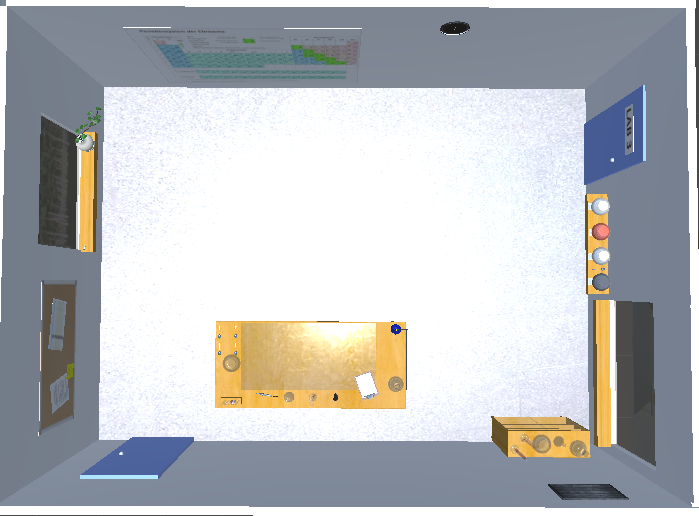
\includegraphics[width=1\textwidth]{images/bisheriger_stand/grundriss_chemielabor.png}
	\caption{Grundriss Chemielabor}
	\label{img:chemielabor}
\end{figure}
\begin{description}
	\item[Flammenf�rbung:]\hfill \\
	Im Raum befinden sich verschiedene L�ffel, ein Bunsenbrenner (auf Grund fehlender Modelle ein Zylinder mit Knopf) und verschiedene Stoffe auf einer Ablage (Calcium, Kalium, Lithium und Kupfer). Man nimmt einen L�ffel, nimmt einen beliebigen Stoff auf, schaltet den Bunsenbrenner an und h�lt den L�ffel in die Flamme. Anschlie�end betrachtet man die gef�rbte Flamme
\end{description}
\begin{description}
	\item[M�llverarbeitung:]\hfill \\
	Der Raum ist angef�llt mit K�rpern aus Styropor. In der Mitte des Raumes befindet sich ein Tisch mit einer Schale voll Aceton. Nimmt man die Styropork�rper auf und wirft sie in die Schale l�sen sie sich nach einiger Zeit auf.
\end{description}
\begin{description}
	\item[Leitbarkeitstest:]\hfill \\
	Auf einem Tisch befindet sich ein Beh�ltnis mit Wasser. Durch das Gef�� l�uft ein Draht der einen Lichtschalter und eine Gl�hbirne verbindet. Da destilliertes Wasser keinen Strom leitet bewirkt das Tasten des Schalters im Ausgangszustand nichts. Erst muss ein leitbarer Stoff, in diesem Fall Salz dem Wasser hinzugegeben werden. Anschlie�end l�sst sich die Lampe einschalten.
\end{description}

Das Git-Repository (vgl. \cite{VSL}) des bestehenden Projektes wurde fortgesetzt. Dort l�sst sich neben der aktuellsten Version auch der Ausgangsstand vor Projektbeginn herunterladen. Dieses ist die Version 1.0 vom 15. August 2019, zu finden im Projekt unter Releases.